\documentclass{beamer}
\usetheme{McMaster}
\beamertemplatenavigationsymbolsempty 
\usepackage{tikz}
\usepackage[export]{adjustbox} % for left/right justifying images
\title{ChatGPT, procedural generation, and large language models: a history}
\author{jbfink}

% Talk is 2023-05-25 1pm.
% ideas / outline
% Randomness
	% e.g. coin flips
% I-Ching and PKD
% Bibliomancy
% That homework machine book
% Bryon Gysin / WSB cut-up
% Markov chaining
% ELIZA
% oblique strategies?
% that 1980s Racter thing and Policeman's Beard
% Demo racter in archive.org 
% Rogue and roguelikes
% https://github.com/brexhq/prompt-engineering is EXCELLENT for history and terms and stuff.
% N-gram models (markov chains; demonstrate dadadodo)
% ChatGPT (sigh)
% Labour issues
% 	IBM outsourcing
% Important LLM (including ChatGPT concepts)
%	context size
%	parameters (7b, 13b, 30b, 65b)
%	Training (Lora, RLHF, few-shot, zero-shot) 
%	Temperature and those other llama.cpp variables (which I think are
%	common to all LLMs)
%	The Prompt
% Other proprietary LLMs (slightly less exasperated sigh)
%	Bard? Anthropic? BERT/RoBERTa?
% Open Source LLMs
% 	Meta's LLaMa
% 	LlaMa Leak
%	Hugging Face
%	Everything else!!!!
%	Non-LLaMa models
% 		StarCoder, RedPajama, etc. etc. etc.
%	Two ways to run local
%		CPU vs GPU
% 		emphasize that CPU is *many factors slower* than GPU
%	Demo llama.cpp
% 	EU's AI act? 
\begin{document}
\begin{frame}
    \maketitle
\end{frame}

\begin{frame}{So many disclaimers}
\begin{itemize}
	\item procrastination
	\pause
	\item English major
	\pause
	\item wtf
\end{itemize}
\end{frame}

 
 \begin{frame}
 	What is \textit{randomness}?
 \end{frame}

\begin{frame}[c]
	\centering
	\Huge
	Yijing / I-Ching
	
	(1000-750 BC)
\end{frame}
  
  \begin{frame}[plain]
  	\makebox[\linewidth]{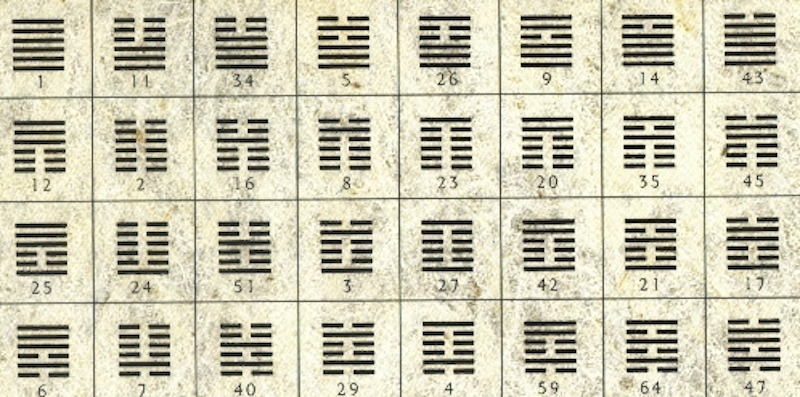
\includegraphics[width=\paperwidth,height=\paperheight]{i-ching.jpg}}
  \end{frame}
  \begin{frame}[c]
  	\centering
  	\Huge
  	The Man in the High Castle
  	
  	(1962)
  \end{frame}

\begin{frame}[plain]
	\makebox[\linewidth]{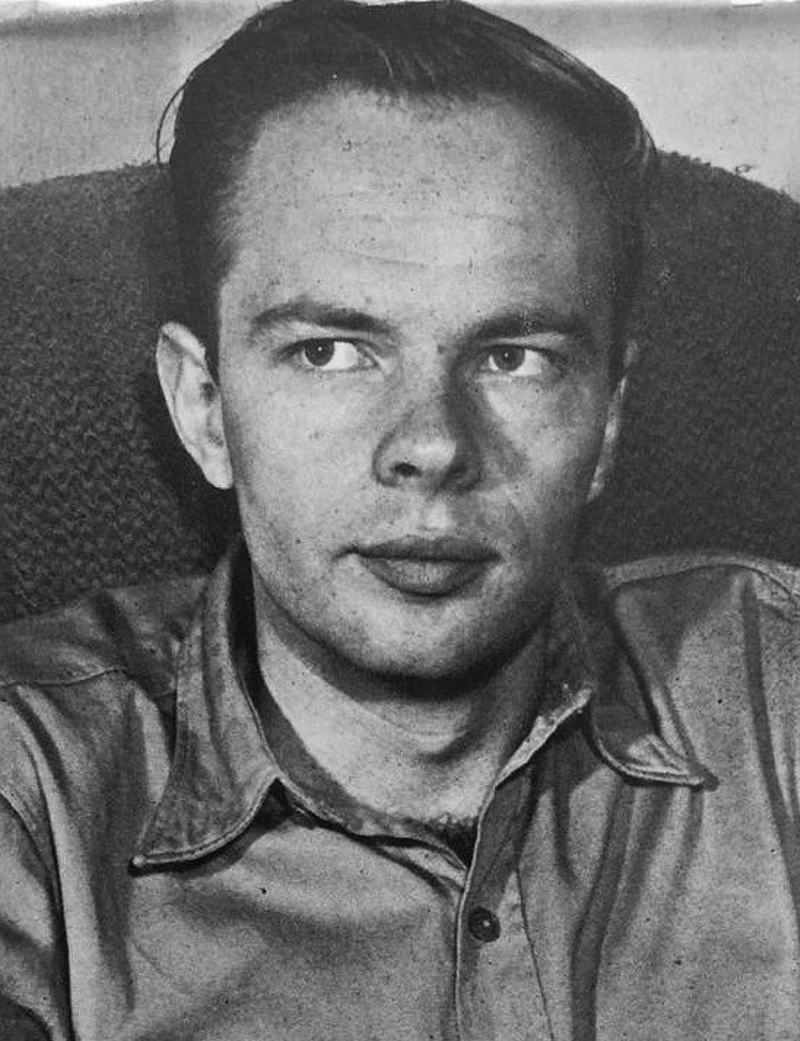
\includegraphics[height=\paperheight]{pkd.jpg}}
\end{frame}

\begin{frame}[c]
	\centering
	\Huge
	Bibliomancy
	
	(1753 - as a term)
\end{frame}

\begin{frame}[plain]
	\makebox[\linewidth]{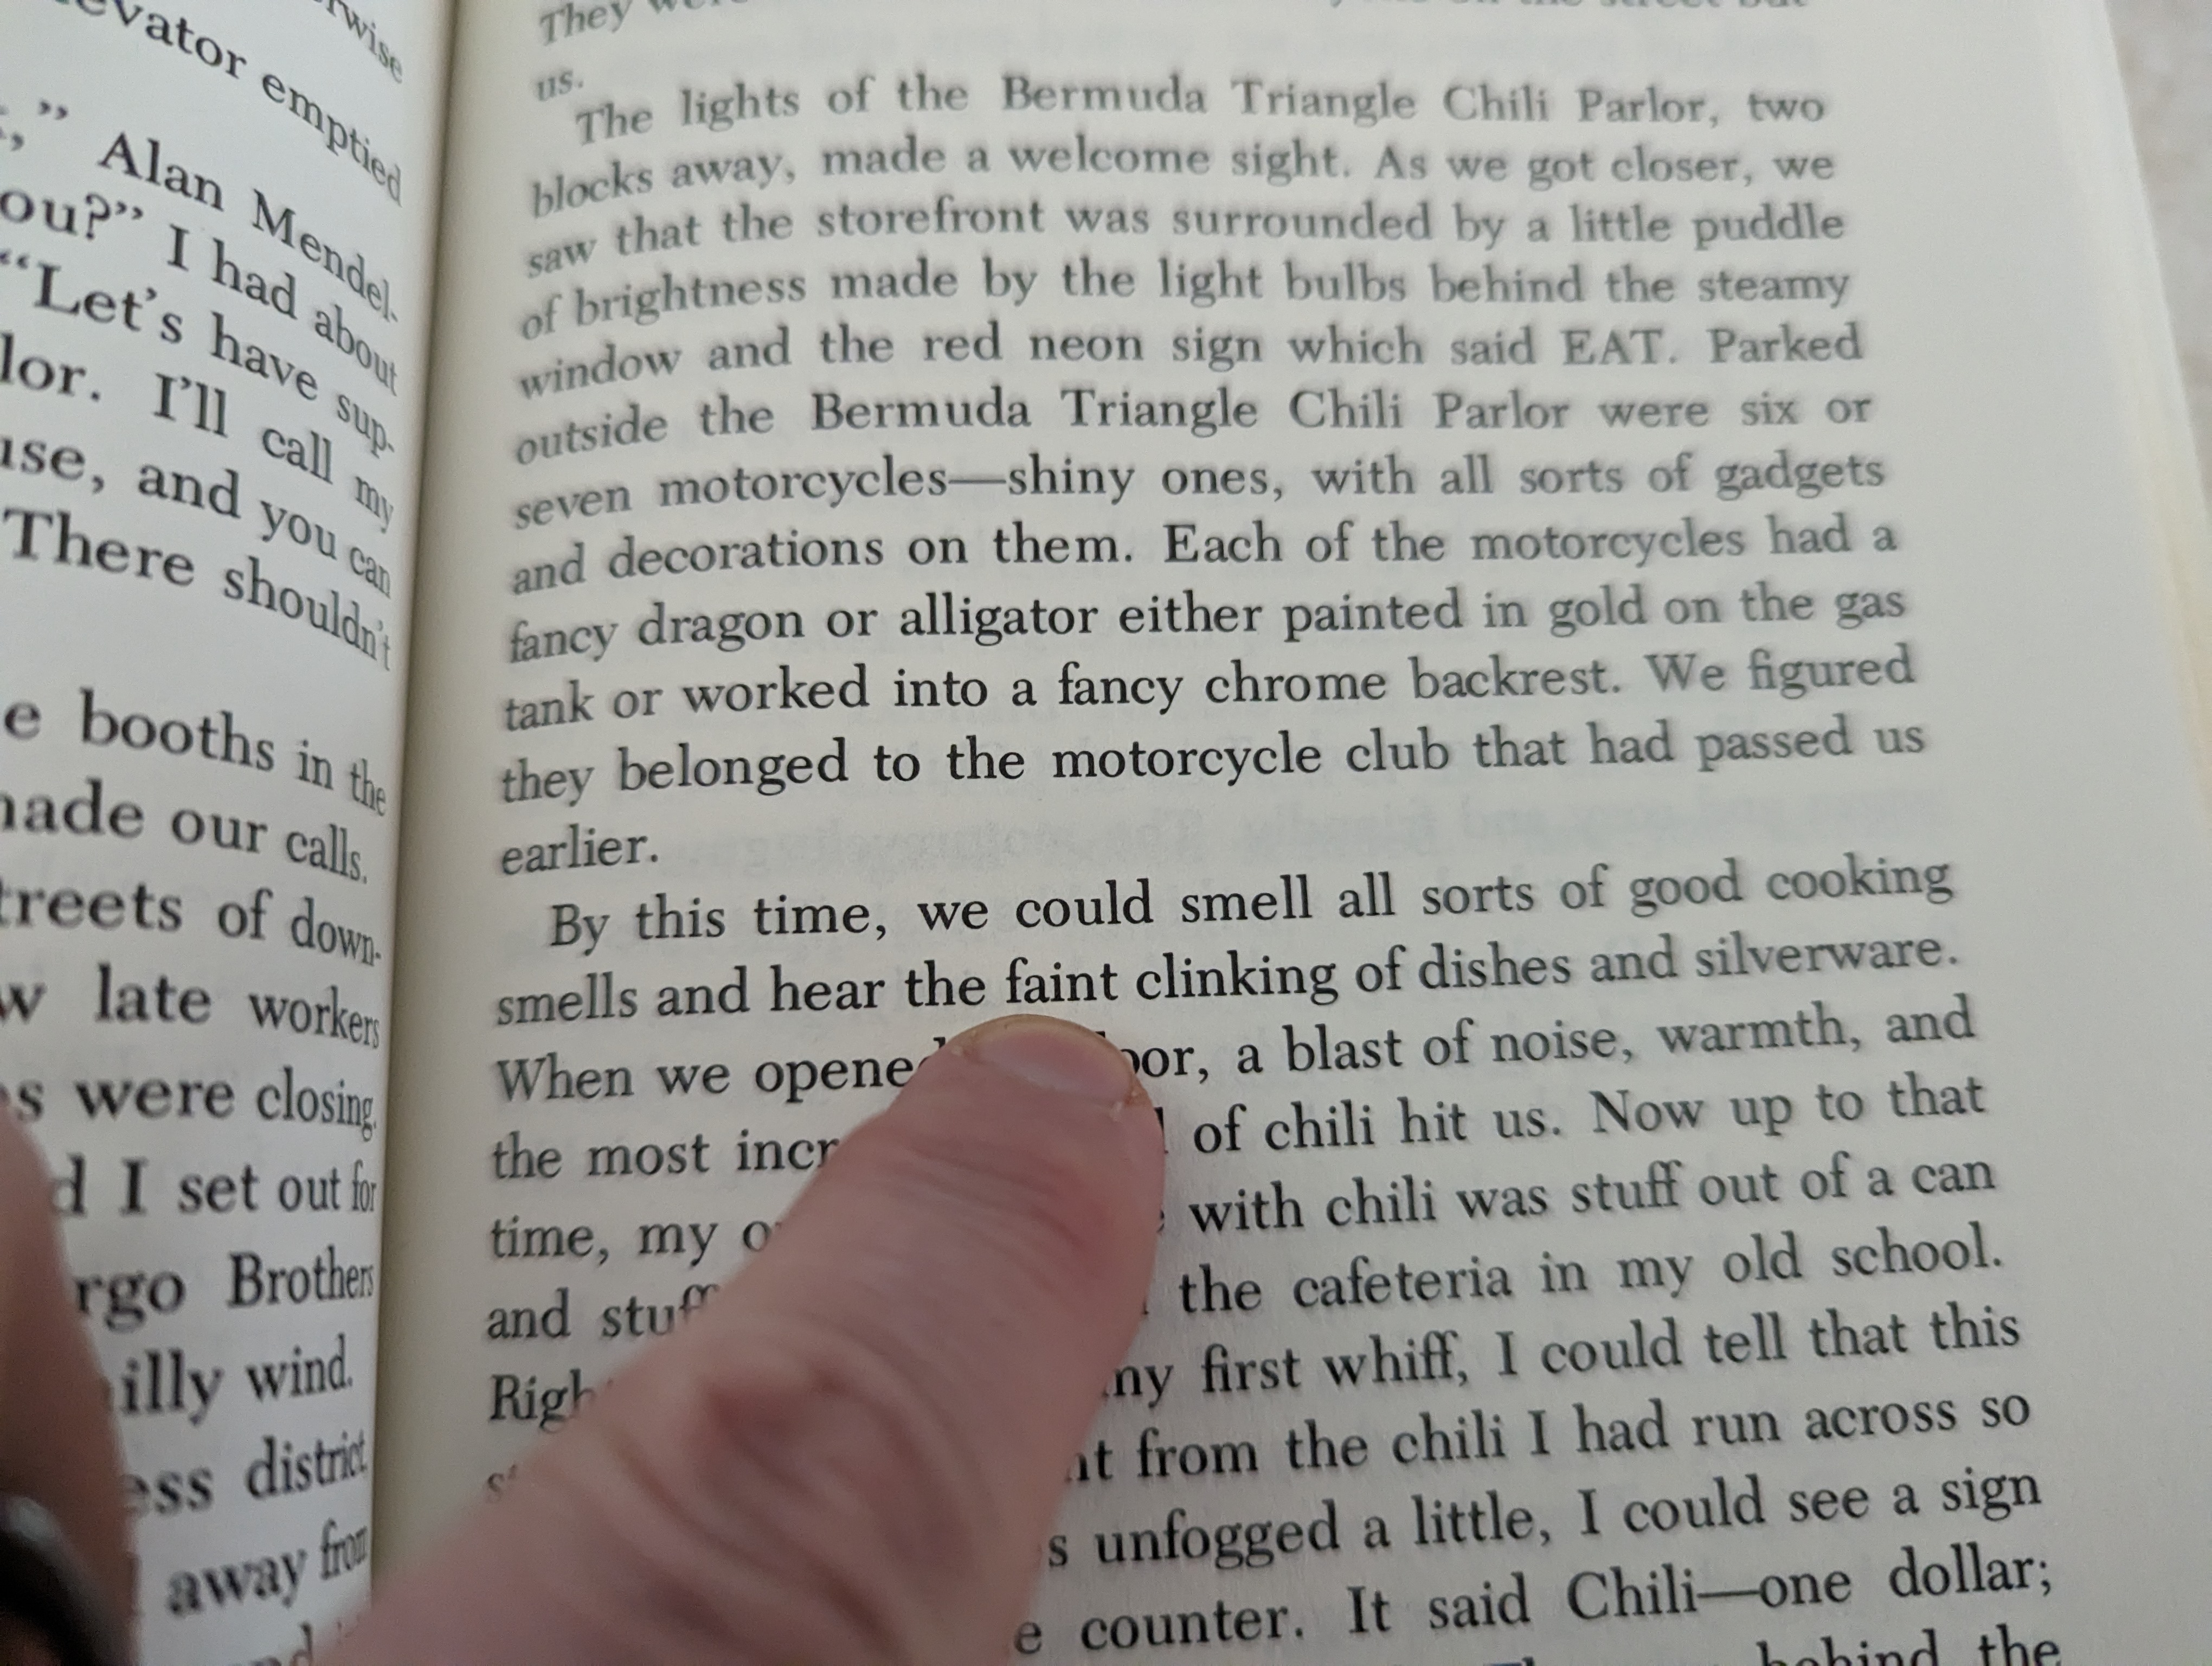
\includegraphics[width=\paperwidth,height=\paperheight]{pinkwater-bibliomancy.jpg}}
\end{frame}

\begin{frame}[c]
	\centering
	\Huge
	The Cut-Up Technique
	
	(1920s)
\end{frame}


\begin{frame}[plain]
	\makebox[\linewidth]{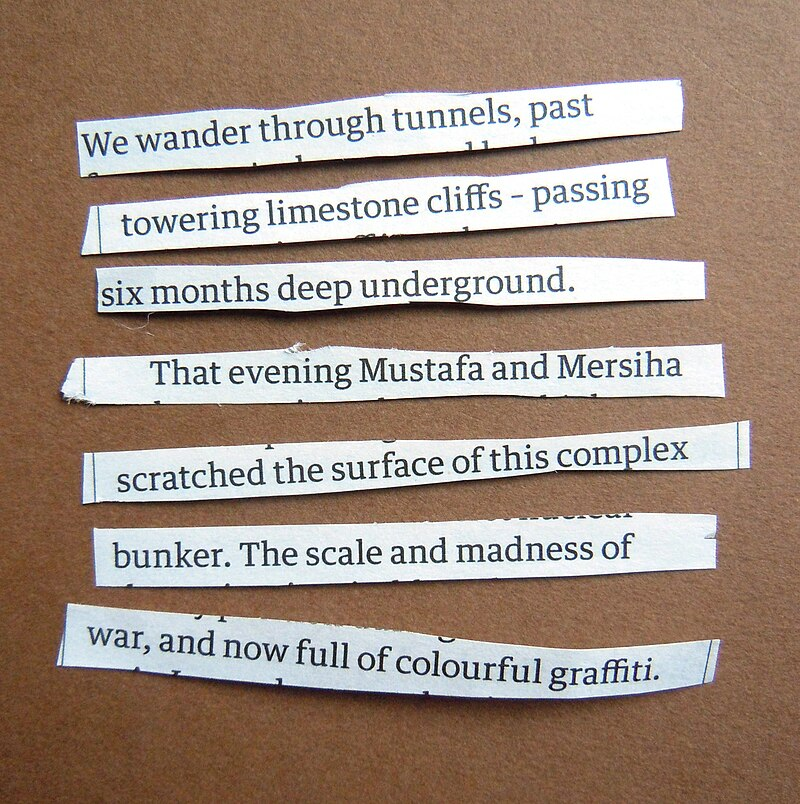
\includegraphics[width=\paperwidth,height=\paperheight]{cut-up.jpg}}
\end{frame}

\begin{frame}[c]
	\centering
	\Huge
	ELIZA
	
	(1966)
\end{frame}

\begin{frame}[plain]
	\makebox[\linewidth]{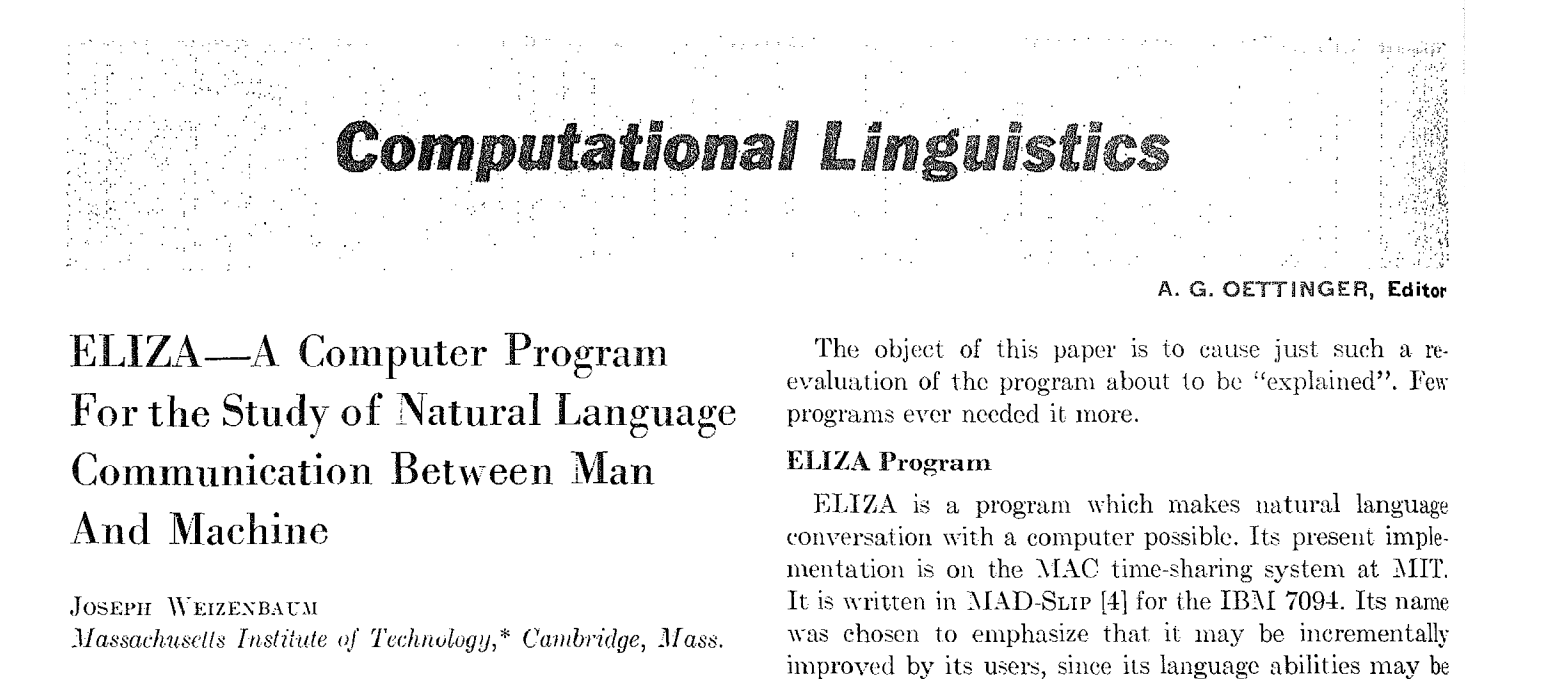
\includegraphics[width=\paperwidth,height=\paperheight]{eliza-paper}}
\end{frame}

\begin{frame}[c]
	\centering
	\Huge
	Oblique Strategies
	
	(1975)
\end{frame}

\begin{frame}[plain]
	\makebox[\linewidth]{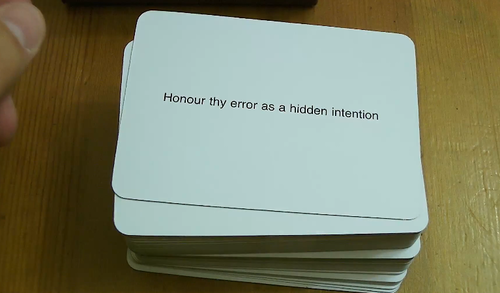
\includegraphics[width=\paperwidth,height=\paperheight]{oblique}}
\end{frame}

\begin{frame}[c]
	\centering
	\Huge
	Rogue
	
	(1980)
\end{frame}

\begin{frame}[plain]
	\makebox[\linewidth]{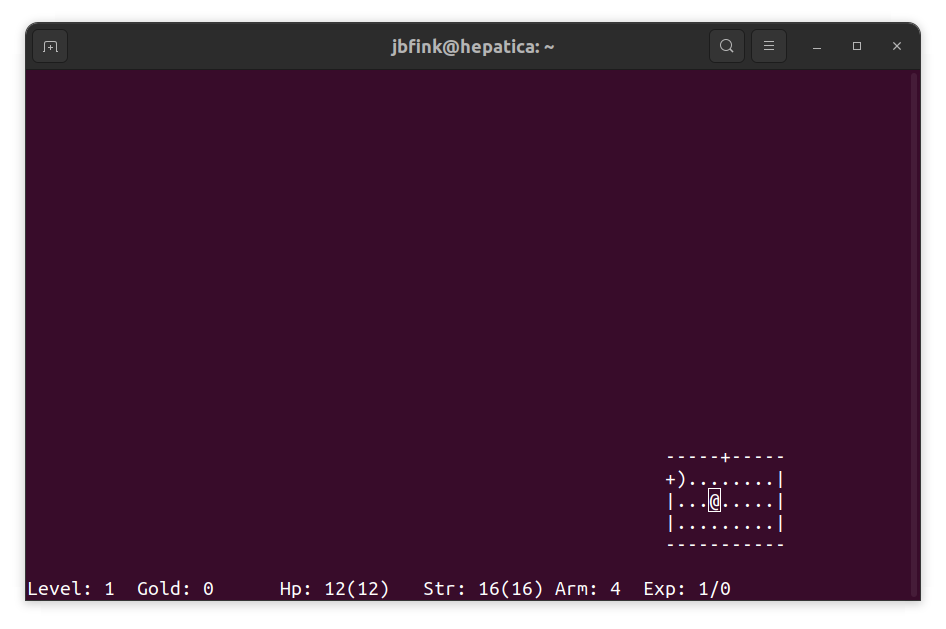
\includegraphics[width=\paperwidth,height=\paperheight]{rogue}}
\end{frame}

\begin{frame}[c]
	\centering
	\Huge
	Murder on the Zinderneuf
	
	(1983)
\end{frame}

\begin{frame}[plain]
	\makebox[\linewidth]{
\includegraphics[width=\paperwidth,height=\paperheight]{zinderneuf}}
\end{frame}

\begin{frame}[plain]
	\makebox[\linewidth]{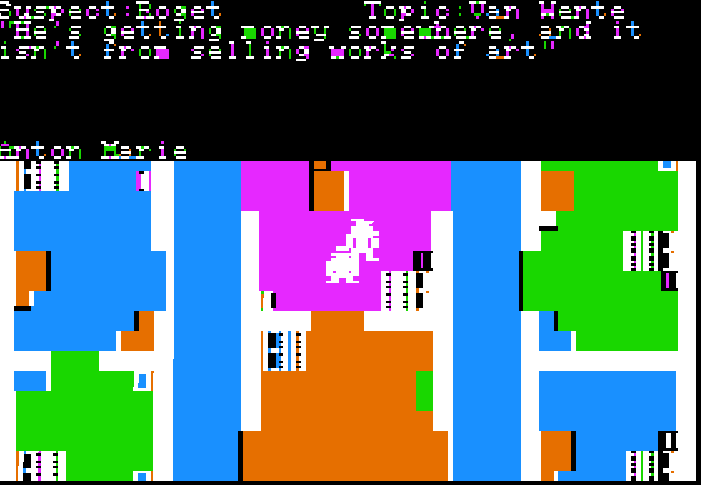
\includegraphics[width=\paperwidth,height=\paperheight]{zinderneuf2}}
\end{frame}

\begin{frame}[c]
	\centering
	\Huge
	Racter and The Policeman's Beard
	
	(1984)
\end{frame}

\begin{frame}[plain]
	\makebox[\linewidth]{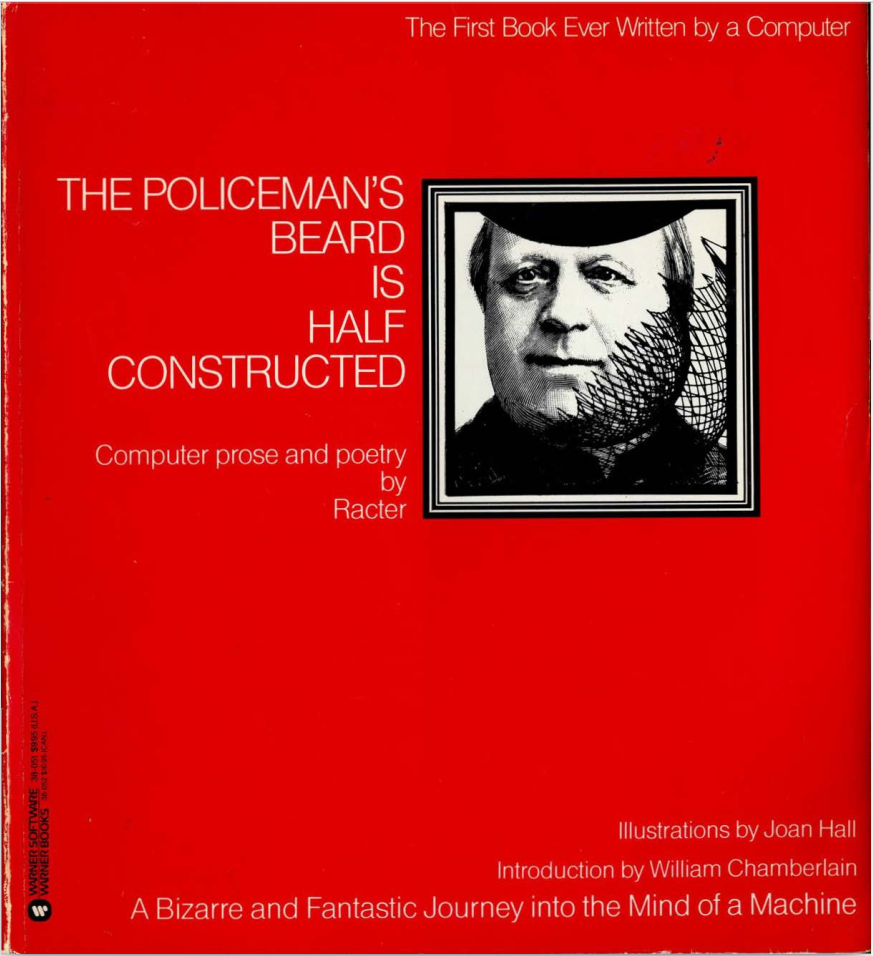
\includegraphics[height=\paperheight]{policemans-beard}}
\end{frame}

\begin{frame}[plain]
	\makebox[\linewidth]{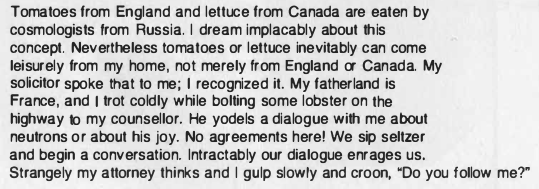
\includegraphics[width=\paperwidth,height=\paperheight]{beard-sample}}
\end{frame}

% racter demo here: run https://archive.org/details/msdos_Racter_1984 in Chrome.

%The 1958 / Danny Dunn thing should probably go right before you actually talk about LLMs

\begin{frame}{so, to recap:}
	\begin{itemize}
		\item 1000BC - Yijing / I-Ching
		\pause
		\item 1000BC-2017AD - some inconsequential stuff happens
	\end{itemize}
\end{frame}

\begin{frame}[c]
	but wait!
	
	\centering
	\Huge
	Danny Dunn and the Homework Machine
	
	(1958)
\end{frame}

\begin{frame}[plain]
	\makebox[\linewidth]{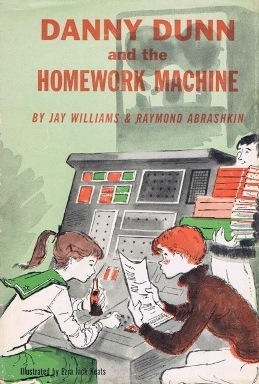
\includegraphics[height=\paperheight]{dannydunn.jpg}}
\end{frame}

\begin{frame}
	A little conversation about the weather.
\end{frame}

\begin{frame}[plain]
	\makebox[\linewidth]{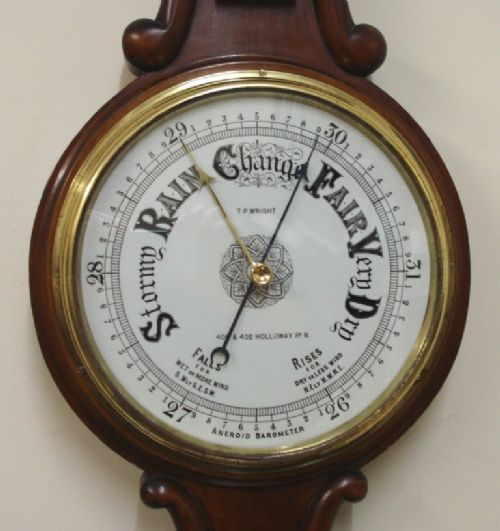
\includegraphics[width=\paperwidth,height=\paperheight]{barometer}}
\end{frame}

\begin{frame}[plain]
	\makebox[\linewidth]{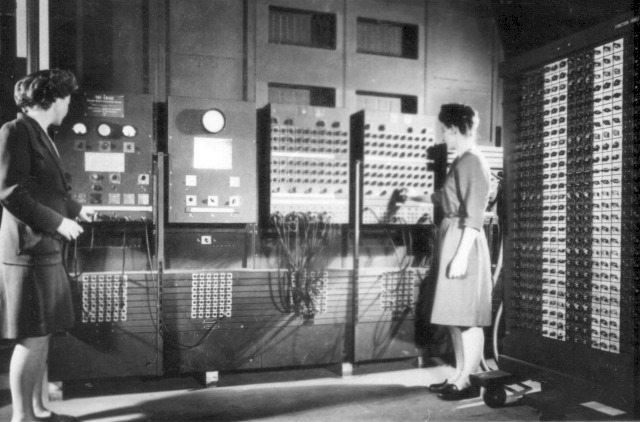
\includegraphics[width=\paperwidth,height=\paperheight]{eniac}}
\end{frame}


\begin{frame}
	Why I say "Large Language Model" and not "AI"
\end{frame}

\begin{frame}
	So, about 2017...
\end{frame}

\begin{frame}[plain]
	\makebox[\linewidth]{
\includegraphics[width=\paperwidth,height=\paperheight]{attention}}
\end{frame}

\begin{frame}{2017-now! Right now!}
	\begin{itemize}
		\item 2017 - "Attention Is All You Need" paper
		\pause
		\item 2018 - "Improving Language Understanding by Generative Pre-Training" paper
		\pause 
		\item 2020 - "Language Models are Few-Shot Learners" paper (GPT-3)
		\pause
		\item 2022 - InstructGPT, and then ChatGPT
		\pause
		\item 2023 - and then....
	\end{itemize}
\end{frame}

\begin{frame}[plain]
	\makebox[\linewidth]{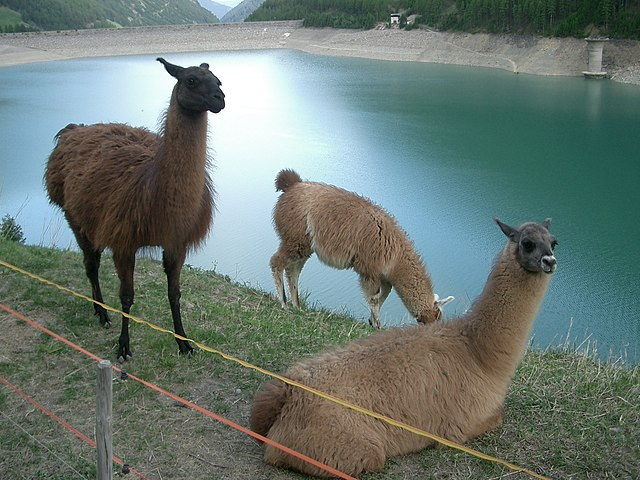
\includegraphics[width=\paperwidth,height=\paperheight]{llamas}}
\end{frame}

\begin{frame}
	"Progress is now moving so swiftly that every few weeks the state-of-the-art is changing or models that previously required clusters to run now run on Raspberry PIs."
	 
	 -- https://github.com/brexhq/prompt-engineering
\end{frame}

\begin{frame}{Important concepts for GPT and other models}
	\begin{itemize}
		\item Context Window and Tokens
		% 2k for LLaMa, 4k for GPT4 chat, 8k/32k via API. This is short term memory.
		\pause
		\item Few-Shot / No-Shot
		\pause
		\item Parameters
		% GPT-1 117m, GPT-2 1.5b, GPT-3 175b, GPT-4 170t 
		\pause
		\item The Prompt, aka "Programming for English Majors"
		\pause
		\item And the Random Seed.
	\end{itemize}
\end{frame}

\begin{frame}
	\begin{itemize}
		\item Context Window is the "memory" of an LLM
		\pause
		\item And Tokens -- words, roughly -- fill up that "memory"
		\pause
		\item And the \textit{response} also takes tokens.
	\end{itemize}
\end{frame}

% demo https://platform.openai.com/tokenizer

\begin{frame}[plain]
	\makebox[\linewidth]{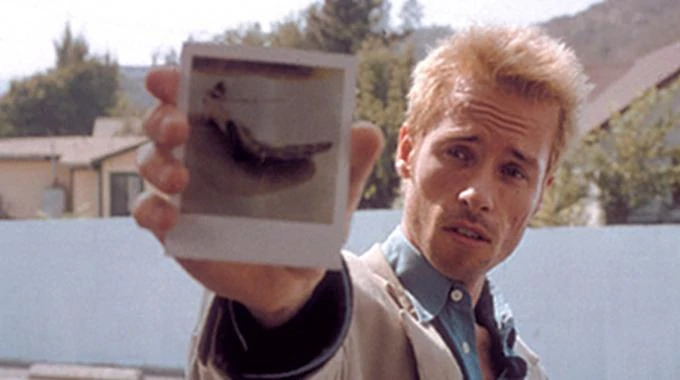
\includegraphics[width=\paperwidth,height=\paperheight]{leonard}}
\end{frame}

\begin{frame}{Few-Shot / No-Shot}
	\begin{itemize}
		\item \textit{Few-Shot} -- a few examples to "teach" an LLM, such as:
		\pause
		\item "I hate it when my phone battery dies." - negative
		\pause
		\item "My day has been great!" - positive
		\pause
		\item "Here is an article." - neutral
		\pause
		\item "This presentation is going fantastic!!!!" - positive
		\pause
		\item And \textit{No-Shot} is exactly what you think it is.
	\end{itemize}
\end{frame}


\begin{frame}{Parameters}
	\begin{itemize}
		\item Roughly corresponds to how "Complex" or "Smart" a model is.
		\pause
		\item (...very roughly)
		\pause 
		\item But \textit{definitely} correlates to resources needed to run the model.
		\pause
		\item Which is why, say, GPT-4 requires this....
	\end{itemize}
\end{frame}

\begin{frame}[plain]
	\makebox[\linewidth]{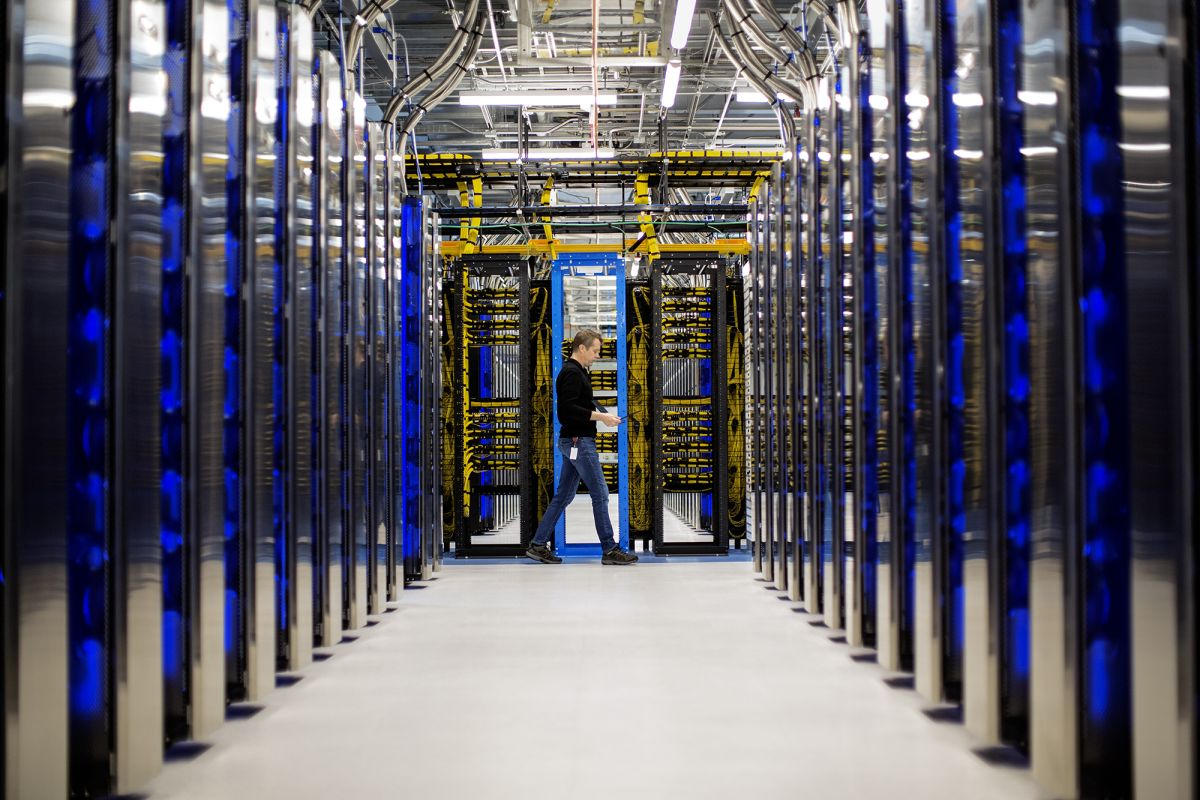
\includegraphics[width=\paperwidth,height=\paperheight]{azure-data-centre}}
\end{frame}

\begin{frame}
	And you can run a 7B model on this....
\end{frame}

\begin{frame}[plain]
	\makebox[\linewidth]{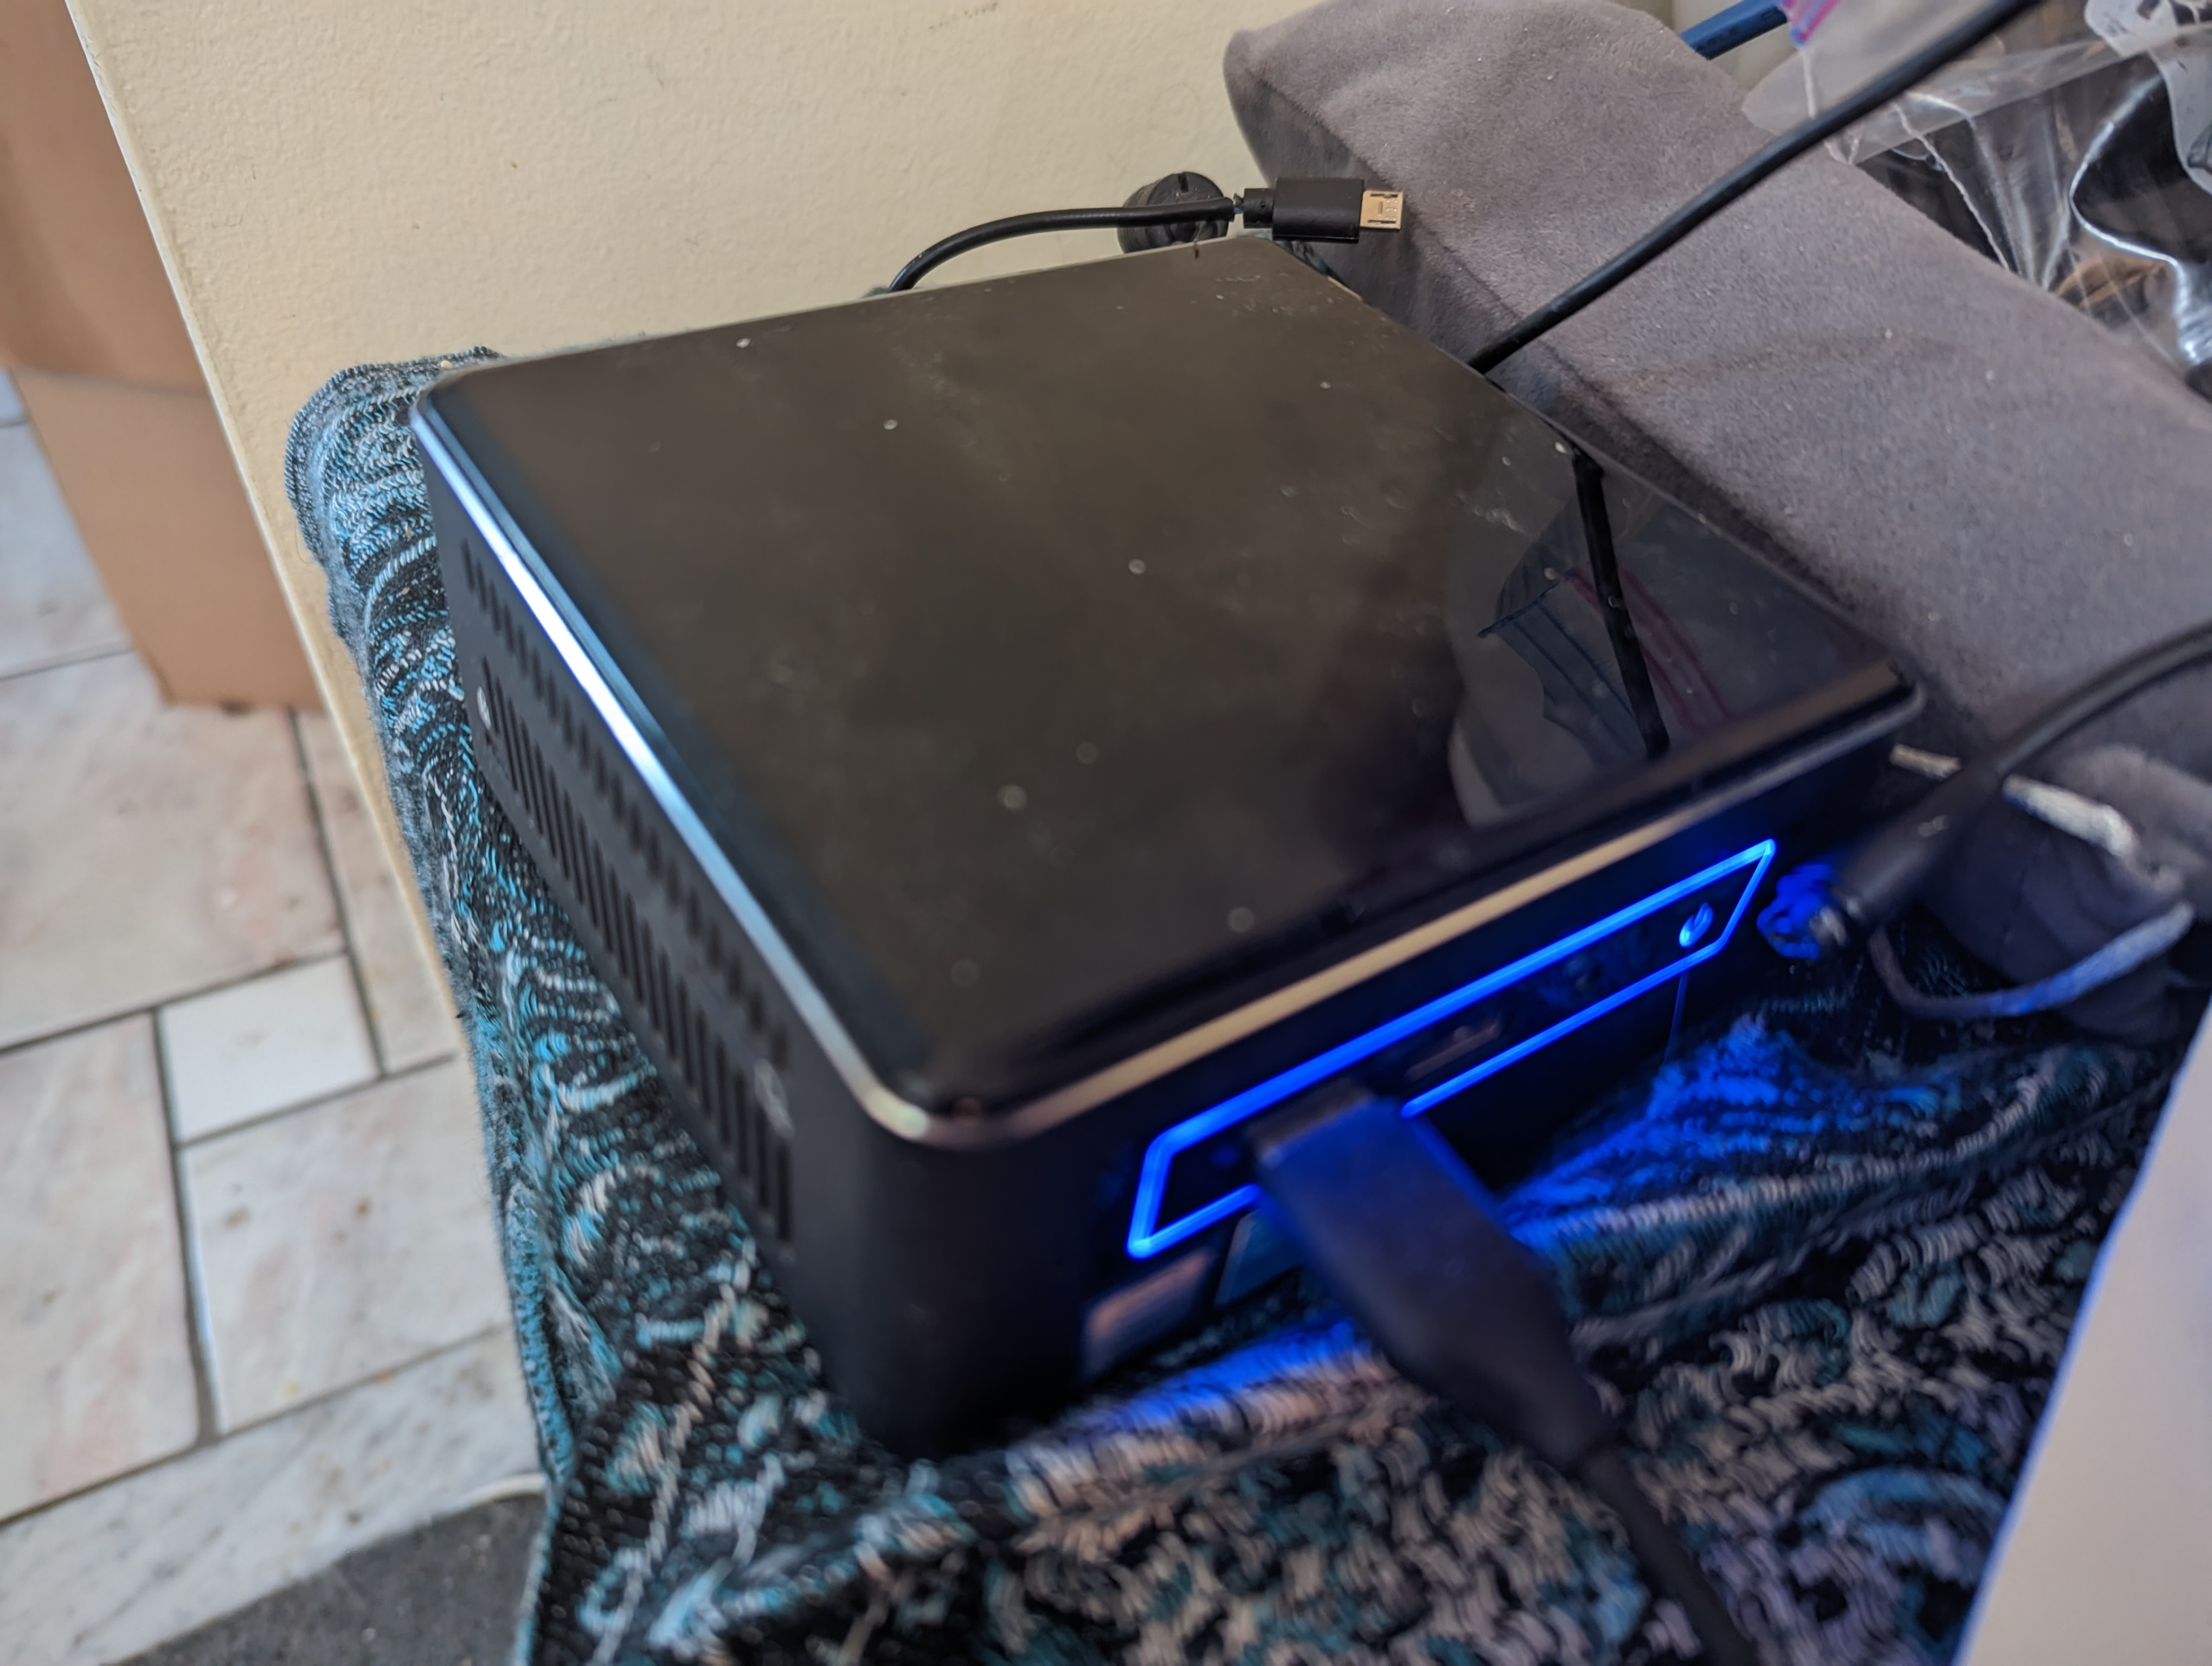
\includegraphics[width=\paperwidth,height=\paperheight]{pfeebe}}
\end{frame}



% demo soup-to-nuts build of llama.cpp on pfeebe:
% git clone https://github.com/ggerganov/llama.cpp
% make clean; make LLAMA_OPENBLAS=1
% copy model file 

% move this slide to *just* before you actually talk about LLMs.
\begin{frame}{things that happened between early May and now}
	\begin{itemize}
		\item llama.cpp breaking changes x2
		\pause
		\item "We Have No Moat"
		\pause
		\item StarCoder
		\pause
		\item Berkeley's OpenLLAMA
		\pause
		\item other
	\end{itemize}
\end{frame}

\begin{frame}{THE FUTURE OF LARGE LANGUAGE MODELS}
	\begin{itemize}
		\item Skynet?
		\pause
		\item ...........
		\pause 
		\item ....larger context windows?s
		
	\end{itemize}
	
	
	
\end{frame}

\begin{frame}
	%this is always the last slide
	Any questions?\\ 
	jfink@mcmaster.ca\\
	
\includegraphics[left, height=4mm]{mastodon} \hspace{1mm}  https://glammr.us/@jbfink
	
\end{frame}

\end{document}
